\documentclass[
  utf8,
  aspectratio=169,
]{beamer}

% === Theme ===
\usetheme{metropolis}

% === Fonts ===
%\usefonttheme{professionalfonts} % overwrite beamer settings
\DeclareUnicodeCharacter{2009}{\,} 
\usefonttheme[]{serif}
\usepackage{noto}
\usepackage{ebgaramond}
%\usepackage[scale=0.75]{sourcecodepro}
\usepackage[cmintegrals,cmbraces]{newtxmath}
\usepackage{ebgaramond-maths}
% Redefining missing symbols
% https://tex.stackexchange.com/questions/215270/can-someone-explain-this-weird-font-behavior-ebgaramond-maths
\makeatletter
  \DeclareSymbolFont{ntxletters}{OML}{ntxmi}{m}{it}
  \SetSymbolFont{ntxletters}{bold}{OML}{ntxmi}{b}{it}
  \re@DeclareMathSymbol{\leftharpoonup}{\mathrel}{ntxletters}{"28}
  \re@DeclareMathSymbol{\leftharpoondown}{\mathrel}{ntxletters}{"29}
  \re@DeclareMathSymbol{\rightharpoonup}{\mathrel}{ntxletters}{"2A}
  \re@DeclareMathSymbol{\rightharpoondown}{\mathrel}{ntxletters}{"2B}
  \re@DeclareMathSymbol{\triangleleft}{\mathbin}{ntxletters}{"2F}
  \re@DeclareMathSymbol{\triangleright}{\mathbin}{ntxletters}{"2E}
  \re@DeclareMathSymbol{\partial}{\mathord}{ntxletters}{"40}
  \re@DeclareMathSymbol{\flat}{\mathord}{ntxletters}{"5B}
  \re@DeclareMathSymbol{\natural}{\mathord}{ntxletters}{"5C}
  \re@DeclareMathSymbol{\star}{\mathbin}{ntxletters}{"3F}
  \re@DeclareMathSymbol{\smile}{\mathrel}{ntxletters}{"5E}
  \re@DeclareMathSymbol{\frown}{\mathrel}{ntxletters}{"5F}
  \re@DeclareMathSymbol{\sharp}{\mathord}{ntxletters}{"5D}
  \re@DeclareMathAccent{\vec}{\mathord}{ntxletters}{"7E}
\makeatother
\renewcommand{\epsilon}{\varepsilon}
\usepackage[]{todonotes}


%\usepackage[osf, sc]{mathpazo}
%\linespread{1.03}
\usepackage{setspace}

\usepackage[T1]{fontenc}
\usepackage{eurosym}
\newcommand{\red}[1]{\colorbox{red}{\textcolor{white}{\textbf{#1}}}}

% === General ===
\usepackage[utf8]{inputenc}
\usepackage{hyperref}
%\usepackage{sfmath}
\usepackage{amsmath}
\usepackage{mathtools}
\usepackage{physics}
\usepackage{siunitx}
\sisetup{per-mode=fraction,fraction-function=\tfrac}
\DeclareSIUnit\gauss{G}
\usepackage[]{braket}
\usepackage{bbm}
\usepackage{threeparttable}
\usepackage{adjustbox}
\usepackage[english]{babel}
\usepackage{eurosym}
\usepackage{epstopdf}
\usepackage{xcolor}
\usepackage{booktabs}
\usepackage{color, colortbl}
\usepackage{array,multirow}
\usepackage{tabularx}
\usepackage{dcolumn}
\usepackage{setspace}
\usepackage{wrapfig}
\usepackage{caption}
\usepackage{subcaption}
\captionsetup{compatibility=false}
%\captionsetup[figure]{labelformat=empty}% redefines the caption setup of the figures environment in the beamer class.
\usepackage{multido}
\usepackage{multicol}
\usepackage{pgf}

\usepackage{listings}
\usepackage{xcolor}
\usepackage[scale=1]{sourcecodepro}
\definecolor{stringcolor}{RGB}{154,91,145}  % rebecca
\definecolor{keywordcolor}{RGB}{80,189,233} % blue
\definecolor{commentcolor}{RGB}{255,0,0}  % red
\lstset{
  basicstyle=\ttfamily\tiny,
  numbers=left,
  breaklines=true,
  language=Python,
  otherkeywords={True,False},
  commentstyle=\color{commentcolor},
  keywordstyle=\color{keywordcolor}\bfseries,
  stringstyle=\color{stringcolor},
  emph={self, csl, ConeShapedCoilArrangement, FieldMap, Collection, Jones_vector},
  emphstyle={\color{keywordcolor}},
}


% === Color theme ===
\makeatletter
\definecolor{lmugreen}{rgb}{0,.58,.25}
\definecolor{lmu-lightgreen}{rgb}{0,.85,.36}
\definecolor{mpqblue}{rgb}{0, .266, 0.371}

\definecolor{thesisred}{RGB}{255,0,0}
\definecolor{thesisgray}{RGB}{71,72,71}
\definecolor{thesisrebecca}{RGB}{105,62,163}
\definecolor{thesisfuchsia}{RGB}{154,91,145}
\definecolor{thesisblue}{RGB}{80,189,233}

\definecolor{hlgray}{gray}{0.8}
\newcolumntype{A}{>{\columncolor{hlgray}}c}
\setbeamercolor{title}{bg=thesisgray,fg=white}
\setbeamercolor{block title}{bg=thesisgray,fg=white}
\setbeamercolor{frametitle}{bg=thesisgray,fg=white}
\setbeamercolor{normal text}{bg=white,fg=black}
\setbeamercolor{alerted text}{fg=thesisgray}
\setbeamercolor{example text}{fg=green!50!black}
\setbeamercolor{structure}{fg=thesisgray}
\setbeamercolor{background canvas}{parent=normal text}
\setbeamercolor{background}{parent=background canvas}
\setbeamercolor{palette primary}{fg=yellow,bg=yellow}
\setbeamercolor{palette secondary}{use=structure,fg=structure.fg!100!green}
\setbeamercolor{palette tertiary}{use=structure,fg=structure.fg!100!green}
\makeatother

% \AtBeginSection[]{
%   \begin{frame}
%   \vfill
%   \centering
%   \begin{beamercolorbox}[sep=8pt,center,shadow=true]{title}
%     \usebeamerfont{title}\insertsectionhead\par
%   \end{beamercolorbox}
%   \vfill
%   \end{frame}
% }

% === Glossary ===
\usepackage[acronym]{glossaries}
\makeglossaries
\newacronym{bert}{BERT}{Bidirectional Encoder Representations from Transformers}
\newacronym{lda}{LDA}{Latent Dirichlet allocation}
\newacronym{nlp}{NLP}{natural language processing}
\newacronym{pca}{PCA}{principal component analysis}
\newacronym{ses}{SES}{socioeconomic status}
\newacronym{tsne}{tSNE}{$t$-distributed stochastic neighbor embedding}


\begin{document}
%%% Title frame
\begin{frame}
	\begin{center}
		\begin{block}
			{\centering\\
				\medskip
				\textbf{\textsc{Idols and Socioeconomic Status}}\\
                Exploring Role Models using Natural Language Processing\\
				\medskip}
		\end{block}

		\bigskip

		Bachelors's thesis discussion\\
		\medskip
		February 20, 2023\\

		\vspace{1cm}
		\textbf{Maximilian Schattauer}
	\end{center}
\end{frame}


%%% Hook
\begin{frame}
	\begin{figure}
		\centering
		
\includegraphics[scale=0.6]{img/lesch.png}
		\caption*{\tiny source: \href{https://bilder.fernsehserien.de/gfx/bv/alpha-centauri.jpg.webp}{https://bilder.fernsehserien.de/gfx/bv/alpha-centauri.jpg.webp}}
	\end{figure}
    
\end{frame}


%%% Overview
\begin{frame}
	\frametitle{Overview}
	\begin{center}
		\textbf{\textsc{Idols and Socioeconomic Status}}\\
		Exploring Role Models using Natural Language Processing\\
	\end{center}
	\vspace{0.5cm}
    \begin{enumerate}
        \item Role Models and SES
        \item Data and Methods
        \item Findings
        \item Discussion
    \end{enumerate}
\end{frame}


%%% Role Models & SES
\begin{frame}
    \frametitle{Role Models and SES}
	\begin{columns}[t]
		\centering
		\begin{column}{0.3\textwidth}
			\onslide<1->{\textbf{Role Models}}
			\begin{itemize}
				\item<2-> child development
				\item<3-> prosocial behavior
				\item<4-> education \& career
			\end{itemize}
		\end{column}
		\begin{column}{0.00\textwidth}<7->
			$\overset{?}{\longleftrightarrow}$
		\end{column}
		\begin{column}{0.35\textwidth}
			\onslide<5->{\textbf{SES}}
			\onslide<6->{\begin{itemize}
				\item child development
				\item prosocial behavior
				\item education \& career
			\end{itemize}}
		\end{column}
	\end{columns}
	\onslide<7->{\begin{center}
		\textbf{$\rightarrow$ interaction effects between role models and SES?}
	\end{center}}

	\onslide<8->{Role model influence determined by:}
	\begin{itemize}
		\item<8-> gender, ethnicity, domain
		\item<9-> relatability \& proximity (mentors vs. celebrities)
	\end{itemize}
	
	\vspace{.2cm}
	\onslide<10->{\textit{This thesis}: self-selected celebrity role models perceived exclusively through media}
\end{frame}


%%% Data and Methods
\begin{frame}
	\frametitle{Data \& Methods}
	\textbf{Data:}
	\begin{itemize}
		\item<+-> survey data: adolescents' (341) SES (low/high) and celebrity role models (184)
		\item<+-> online newspaper articles
	\end{itemize}
	\onslide<+->{
		\textbf{Objectives: }
		\begin{itemize}
			\item finding differences between reports about low-SES and high-SES role models
			\item testing applicability of NLP methods in social economics
		\end{itemize}
	}
	\onslide<+->{
		\textbf{Foci of analysis:}
		\begin{itemize}
			\item distribution of topics
			\item sentiment
			\item connotations of relatability, success, and behavior
			\item journalistic aspects
		\end{itemize}
	}
\end{frame}
\begin{frame}
	\frametitle{Data \& Methods (cont.)}
	\textbf{NPL techniques:}
	\begin{itemize}
		\item <+-> topic modelling:
		\begin{figure}
			\centering
			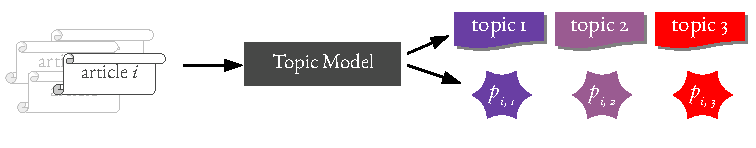
\includegraphics[scale=1]{img/topic_modelling_schema_simple.pdf}
		\end{figure}
		\item <+-> zero-shot classification:
		\begin{figure}
			\centering
			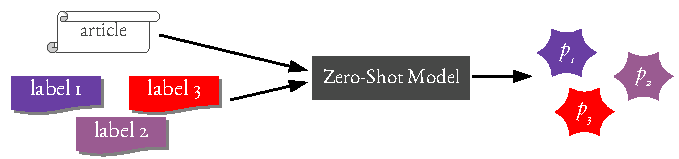
\includegraphics[scale=1]{img/zero_shot_schema_simple.pdf}
		\end{figure}
	\end{itemize}
\end{frame}


%%% Findings
\setbeamercovered{transparent}
\begin{frame}
	\frametitle{Findings}
	\begin{columns}[t]
		\begin{column}{0.18\textwidth}
			\begin{itemize}
				\item<1> topics
				\item<2> sentiment
				\item<3> prosociality
				\item<4> crime
			\end{itemize}
		\end{column}
		\begin{column}{0.82\textwidth}
			\only<1>{
				\begin{figure}
					\resizebox{7cm}{!}{../../presentation/img/semantic_clustering_hypertopic_distribution_distinct.pgf}
				\end{figure}
			}
			\only<2>{
				\begin{figure}
					\resizebox{7cm}{!}{../../presentation/img/zero_shot_distribution_sentiment_n_distinct.pgf}
				\end{figure}
			}
			\only<3>{
				\begin{figure}
					\resizebox{7cm}{!}{../../../build/thesis/70-supervised/zero_shot_distribution_prosociality_distinct.pgf}
				\end{figure}
			}
			\only<4>{
				\begin{figure}
					\resizebox{7cm}{!}{../../presentation/img/zero_shot_distribution_crime_type_distinct.pgf}
				\end{figure}
			}
		\end{column}
	\end{columns}
\end{frame}
\setbeamercovered{invisible}

%%% Discussion
\begin{frame}
	\frametitle{Discussion}
	\textbf{Findings:}
	\begin{itemize}
		\item<1->[\checkmark] found significant and interpretable differences between low- and high-SES role model reports
		\item<2->[\checkmark] showed example of NLP application in social economics
	\end{itemize}

	\onslide<3->{\textbf{Validity \& Potential Improvements:}}
	\begin{itemize}
		\item<3->[!] data abundance and variety
		\item<4->[!] aggregation strategy
		\item<5->[!] model tuning
	\end{itemize}

	\onslide<6->{\textbf{Outlook:}}
	\begin{itemize}
		\item <6->{Future of the survey participants?}
		\item <6->{Other applications of NLP in economics?}
	\end{itemize}
\end{frame}
\end{document}